\chapter{Surface Heat Flux}

CFAST includes calculation of heat flux via convection, radiation, and conduction to compartment surfaces and targets. Heat transfer to the inside surface of compartment linings and the front and rear faces (as specified by the user) of targets consists of convection (through the use of empirical correlations) and radiation (calculated by the model using view factors for the fire, gas layers, and compartment surfaces). Heat conduction into a solid surface is calculated via a one-dimensional solution of the heat equation in cartesian or cylindrical coordinates.  The latter is particularly useful for predicting the thermal response of electrical cables.

For compartment linings, the ``outside'' surface is, by default, exposed to the exterior ambient temperature with convection and radiation calculated in a similar manner to the inside surface.  The ``outside'' boundary condition can also be specified as a constant temperature (i.e., the outside surface can be at ambient temperature) or can be connected to the ``outside'' surface of part or all of a second compartment.  For targets, the back surface is simply pointed in a direction opposite that of the front surface with convection and radiation calculated in a similar manner to the front surface. This chapter contains a variety of heat flux measurements, ranging from less than a kW/m$^2$ from very small gas burners  to more than 100~kW/m$^2$ in full-scale compartment fires.

\section{Heat Flux to  Compartment Ceiling, Wall, and Floor Surfaces}

In the NIST/NRC tests, heat flux gauges and thermocouples were positioned at various locations on the walls, floor, and ceiling of the fire compartments. The locations are given in Table~\ref{NIST_NRC_Wall_Coords}. The heat flux gauges were not water cooled; thus, they measured the {\em net} rather than the {\em gauge} heat flux. However, the net heat flux is a function of the temperature of the heat flux gauge itself, which is not something that is modeled. To better compare model and measurement, the measured net heat flux is converted into a gauge heat flux using the following formula:
\begin{equation}
\dot{q}''_{\subscript{gauge}} = \dot{q}''_{\subscript{net}} + \sigma \left( T^4_{\subscript{gauge}} - T^4_\infty \right) + h  \left( T_{\subscript{gauge}}-T_\infty \right) \quad \hbox{kW/m}^2
\end{equation}
where $\sigma=5.67 \times 10^{-11}$~kW/m$^2$/K$^4$ and $h=0.005$~kW/m$^2$/K.

Also, over the course of 15 experiments, numerous heat flux gauges failed, most often due to loss of contact with the wall or faulty thermocouples. All of the measurements from Test~13 and 16 were found to be flawed.

In the WTC tests, there were a variety of heat flux gauges installed in the test compartment. Most were within 2~m of the fire. Their locations and orientations are listed in Table~\ref{WTC_Gauges}. This section contains the measurements at the floor and ceiling.

\begin{table}[h!]
\caption{Heat flux gauge positions relative to the center of the fire pan in the WTC series.}
\begin{center}
\begin{tabular}{|l|c|c|c|c|l|}
\hline
Name    & $x$ (m)   & $y$ (m) & $z$ (m)   & Orientation  & Location  \\ \hline \hline
H2FU    & 0.64      & 0.63    & 3.30      &     $+z$     & Truss Support         \\ \hline
H2RU    & 0.64      & 0.51    & 3.30      &     $+z$     & Truss Support          \\ \hline
H2FD    & 0.64      & 0.30    & 3.15      &     $-z$     & Truss Support          \\ \hline
H2RD    & 0.64      & 0.42    & 3.15      &     $-z$     & Truss Support          \\ \hline
HCoHF   & -0.90     & 0.84    & 3.46      &     $+x$     & Column, facing fire          \\ \hline
HCoHW   & -0.97     & 0.92    & 3.27      &     $+y$     & Column, facing north          \\ \hline
HCoLF   & -0.90     & 0.84    & 0.92      &     $+x$     & Column, facing fire          \\ \hline
HCoLW   & -0.97     & 0.92    & 1.02      &     $+y$     & Column, facing north          \\ \hline
HF1     & 1.06      & 0.13    & 0.13      &     $+z$     & Floor          \\ \hline
HF2     & 1.56      & 0.10    & 0.13      &     $+z$     & Floor          \\ \hline
HCe1    & -0.45     & 0.35    & 3.82      &     $-z$     & Ceiling          \\ \hline
HCe2    &  0.05     & 0.35    & 3.82      &     $-z$     & Ceiling          \\ \hline
HCe3    &  0.80     & 0.35    & 3.82      &     $-z$     & Ceiling          \\ \hline
HCe4    &  2.56     & 0.35    & 3.82      &     $-z$     & Ceiling          \\ \hline
\end{tabular}
\end{center}
\label{WTC_Gauges}
\end{table}

Figure \ref{fig:Surface_Flux_Scatter} shows a comparison of predicted and measured values for total heat flux. Appendix B provides comparisons of heat flux and surface temperature on cable and surface targets.
\label{Target Heat Flux}

\begin{figure}
\begin{center}
\includegraphics[width=4in]{FIGURES/ScatterPlots/Surface_Heat_Flux}
\end{center}
\caption{Comparisons of Measured and Predicted Compartment Heat Flux to Surfaces} \label{fig:Surface_Flux_Scatter}
\end{figure}


\section{Heat Flux to Targets}

In the NIST/NRC tests, cables in various types (power and control), and configurations (horizontal, vertical, in trays or free-hanging), were installed in the test compartment. For each of the four cable targets considered, measurements of the radiative and total heat flux were made with gauges positioned near the cables themselves.  In the WTC tests, There were a variety of heat flux gauges installed in the test compartment. Most were within 2~m of the fire. Their locations and orientations are listed in Table~\ref{WTC_Gauges}. Figure \ref{fig:Target_Flux_Scatter} shows a comparison of predicted and measured values for total heat flux. Appendix B provides comparisons of heat flux and surface temperature on cable and surface targets.
\label{Surface Heat Flux}
\label{Wall Heat Flux}
\label{Ceiling Heat Flux}
\label{Floor Heat Flux}

\begin{figure}
\begin{center}
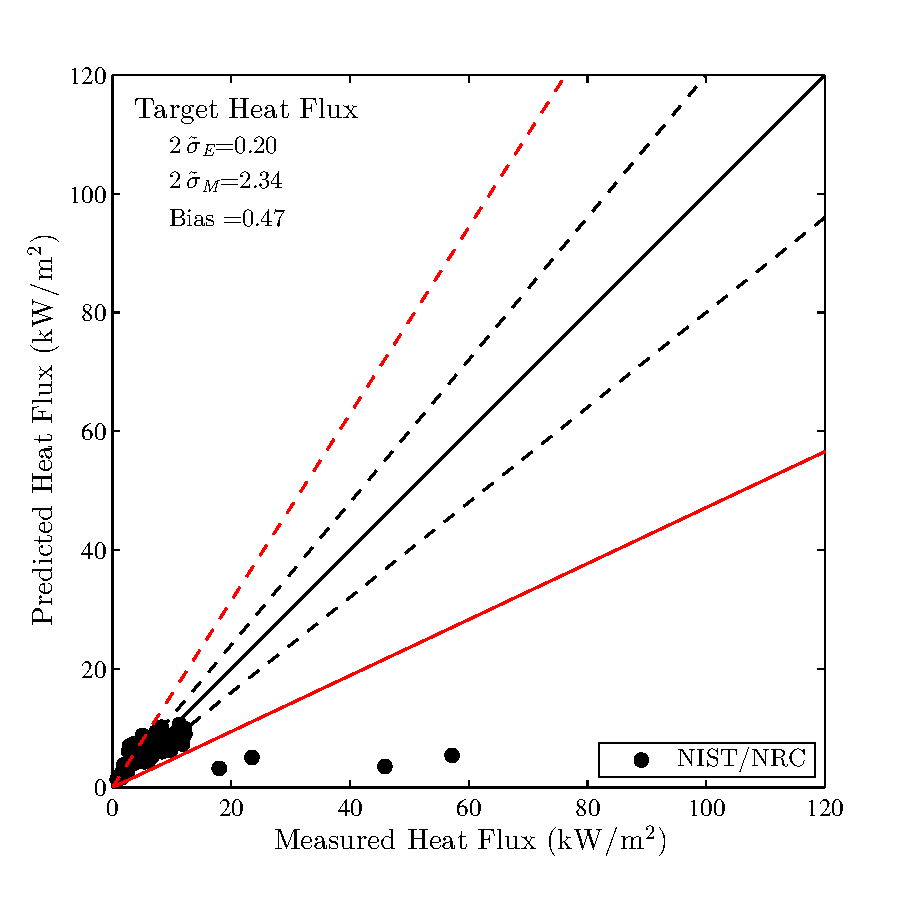
\includegraphics[width=4in]{FIGURES/ScatterPlots/Target_Heat_Flux}
\end{center}
\caption{Comparisons of Measured and Predicted Heat Flux to Targets} \label{fig:Target_Flux_Scatter}
\end{figure}

